\section{Results}

% 1 page
%Renan: Results-Intro
%TODO Gabriel: Results-Calibration
%Estevão: Results-Mecanica
%Renan: Results-Control

% Intro

Simulations and experimental tests were performed to verify the proposed
concepts. The following results were divided according to the EMMA system's
elements introduced in Sec.~\ref{solution}. 


\subsection{Robotic manipulator analysis}\label{sec::man_analysis}

As stated in Subsec.~\ref{manipulator}, simulations for the robotic
manipulator were implemented with OpenRave, and consist of the following steps:
blade's surface discretization; coating strategy; coating segmentation
(partitioning) and base positions computation; kinematics, dynamics and
manipulability.

The blade's surface discretization is an uniform sampling of the blade to
determine where to the coating directions should be. However, sampling the
actual geometric surface can lead to unwanted results due to possible
concavities. A simpler approach is to take the bounding box of the blade and
sample its surface uniformly (\textit{axis-aligned bounding box}). Once the
surface of the box is sampled, the intersection of the blade and a ray
originating from each point going inward is taken. The normal of the blade's
surface from each of these intersection points is taken to be the coating
direction. As an uniform sampling of the box does not mean an uniform sampling
of the blade, the box is oversampled and a 50~mm filter is applied to the
resulting sampling of the blade, by a multidimensional search key with k-d tree.
The result is an uniformely sampled blade, and the samples are spaced
50~mm from each other. These samples are translated 230~mm in respect with their
normal vectors, collision checks with the environment are made, and the
feasible samples are named \textit{coating samples}.
Fig.~\ref{fig:discretization} shows blade's discretization and the
\textit{coating samples}. 

\begin{figure}
	\centering
	\subfigure{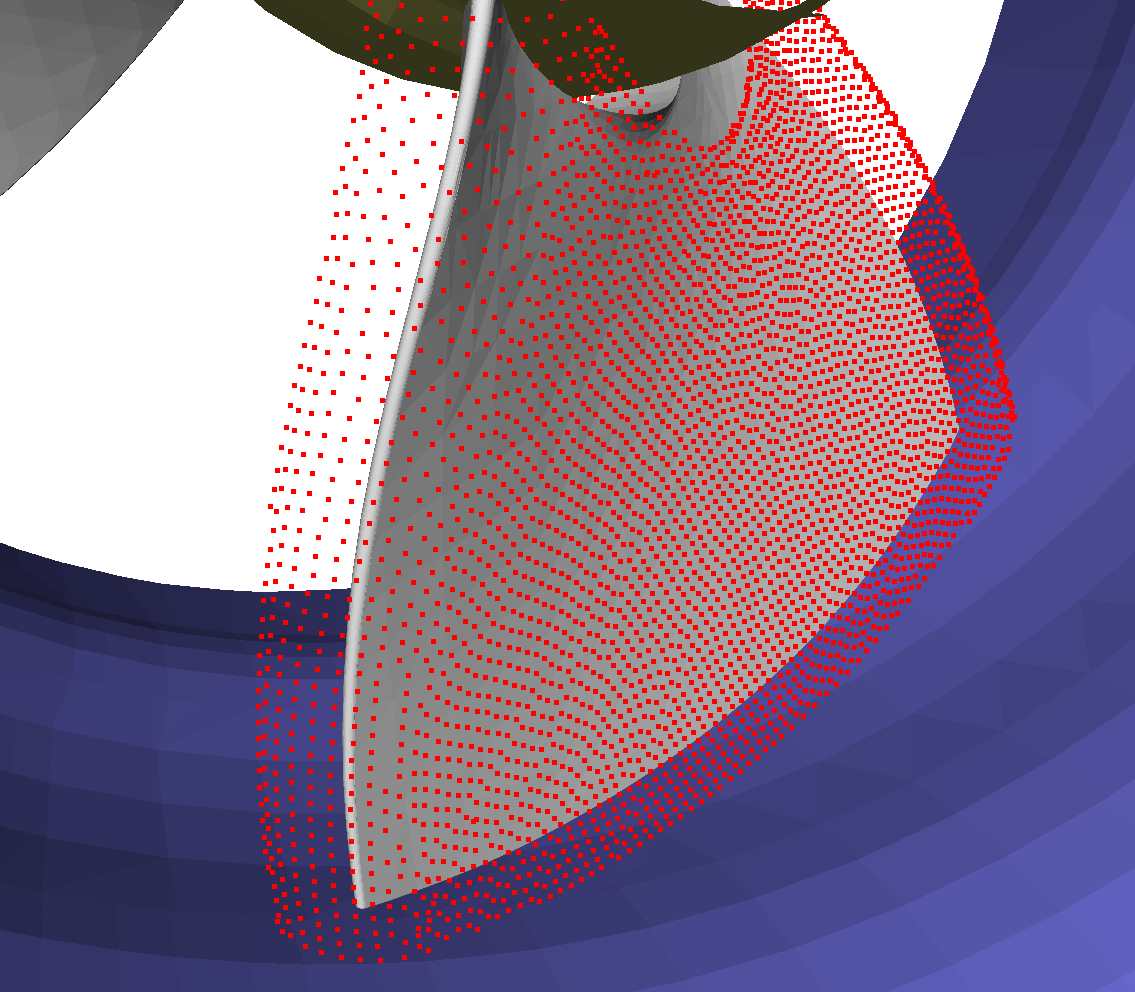
\includegraphics[width=0.47\columnwidth]{figs/results//blade_grid1.png}}\quad
	\subfigure{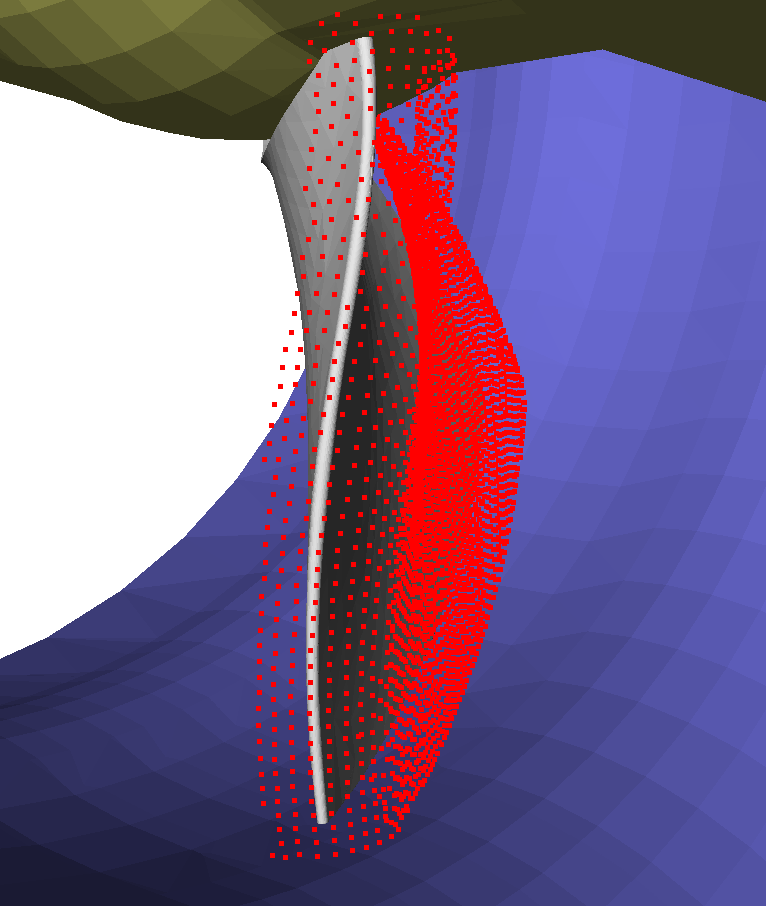
\includegraphics[width=0.47\columnwidth]{figs/results//blade_grid2.png}}
    \label{fig:discretization}
    \caption{Blade discretization and \textit{coating samples} in red}
\end{figure}

The coating segmentation and base positions computation is to calculate the
required robotic manipulator's base positions to process all the \textit{coating
samples} with angle and distance tolerances. It is a brute force search, in
which the positions are uniformly sampled in the turbine's confined space. For
each position, inverse kinematics (IKFast) are computed to determine the
robotic manipulator's joint parameters that provide the desired positions and
orientations of the end-effector. Fig.~\ref{fig:coating} shows examples of the
algorithm, where black dots are coated points and blue dots are coated points
with angle tolerance. At the end of the Alg.~\ref{alg:strategy}, the reachable
samples are in the Matrix~\ref{algvar:reachable}, which relates coating samples
with base positions, thus it is possible to create a coating strategy and to
select the simplest base positions. The result is the minimum required
positions for the robotic manipulator's base.

\begin{figure}
	\centering
	\subfigure{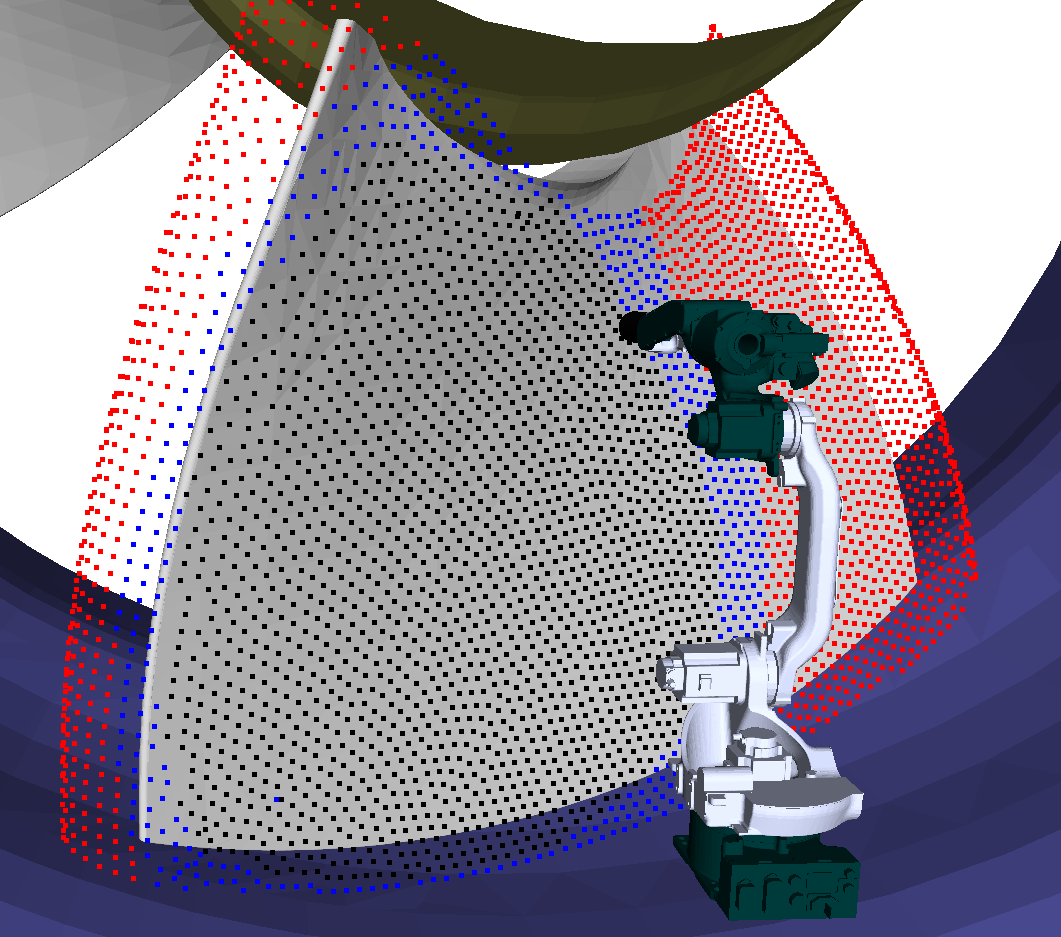
\includegraphics[width=0.47\columnwidth]{figs/results/mh12_coating1.png}}\quad
	\subfigure{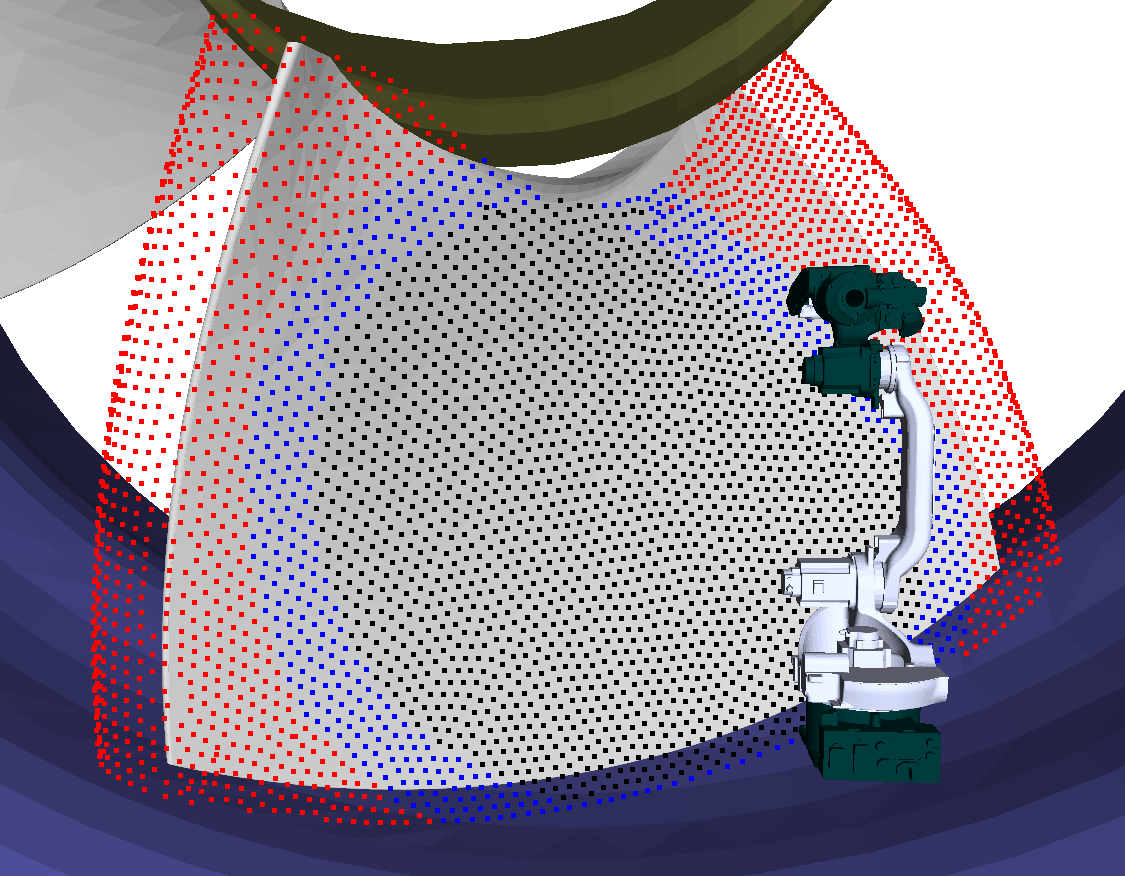
\includegraphics[width=0.47\columnwidth]{figs/results/mh12_coating2.png}}
    \caption{Robotic manipulator coating samples.}
     \label{fig:coating}
\end{figure}

\begin{algorithm}
\caption{Coating strategy}
\label{alg:strategy}
\begin{algorithmic}[1]
\ForAll{Base positions} 
		\ForAll{\textit{Coating samples}}
			\State Joints = IKFast(sample)
			\If{not Joints} 
				\State Joints = IKFast(sample,tol)
			\EndIf
			\If{Joints} 
				\State $\textrm{Reachable}[\textrm{pos}] += [\textrm{sample}]$
				\label{algvar:reachable}
			\EndIf
		\EndFor
\EndFor
\end{algorithmic}
\end{algorithm}

The kinematic approach described above is not enough to ensure that the robot
will reach the \textit{coating samples}. Maximum accelerations, decelerations,
torques, and jacobian singularities should be investigated and compared to the robotic
manipulator's specifications. The Newton-Euler method
\cite{sciavicco2000differential} was adopted for torque computation: $\tau =
M(q)\alpha + C(q,\omega)\omega + G(q)$, where $\tau$ is the joints' torques,
$M$ is the matrix of links' masses and moments of inertia, $\alpha$ is the
joints' accelerations, $q$ is the joints' angles, $\omega$ is the joints'
velocities, $C$ is the Coriolis matrix, and $G$ is the gravity vector.

In the dynamic approach, $M$ was estimated by the robotic manipulator's CAD
model. The angular accelerations are derived by differential kinematics:
$\alpha=J^+(a-\omega^TH\omega)$, where $H$ is the Hessian matrix
\cite{hourtash2005kinematic}, $a=\ddot{X}$ is the linear accelerations, and $J$
is the Jacobian matrix. Therefore, torques can be analytically estimated with
the inverse dynamics in OpenRave. Comparing estimated torques with the technical
specifications, dynamics simulations's results showed that the robotic
manipulator should be placed at, at least, 1400~mm distance from the blade's
surface. Placing the robot nearer would enhance the robotic manipulator's
workspace, but it would increase the torques also, above the technical
specifications. Fig.~\ref{fig:torques} shows joints' torques for blades's
\textit{coating samples} in a color gradient way, where red dots represents
small magnitudes and blue dots large magnitudes. The Fig.~\ref{fig:torques} is
an example of the robotic manipulator in a close range, 900~mm distance from the
blade.

\begin{figure}
	\centering
	\includegraphics[width=.5\columnwidth]{figs/results/manipulability_colorgradient.png}
    \caption{Robotic manipulator joints' torques in color gradient.}
    \label{fig:torques}
\end{figure}

\subsection{Base analysis}
%TODO Estevão: falar o programa utilizado para a análise, numero de elementos
% finitos e parametros necessarios para reproduçao da analise
The FEA analysis of the base verifies the Von Mises stress and displacements
along the structure's slender members. The stress analysis determines the
integrity of the base due to the maximum loads of the robotic manipulator. The
displacements determine if the structure provides a rigid base for the robotic
manipulator. According to the hard coating requirements, big displacements are
not even allowable in the elastic region of the material. 
%TODO Estevão: big displacements é generico. 

The maximum Von Mises stress was 5.78~MPa, which gives a factor of safety of
34.6. It was found for a particular case where the robotic manipulator is in
the secondary rail, 800~mm from the rotational joint. The displacement of the
structure causes a maximum translation of 0.47~mm and a angular deflection of
$0.0149^{\circ}$ in respect to robotic manipulator base's coordinate system. 
%TODO Estevão: figura!

%TODO Estevão: Testes in situ com a base magnética


\subsection{Calibration analysis}

Field tests are very complex due to the logistics and the availability of a dry
hydropower turbine, thus simulated data were analyzed, which can be consistent
and can represent effectively the actual operation scenario. In calibration
analysis, turbine's environment and the robotic manipulator were simulated with
the toolbox Blensor \cite{Gschwandtner11b}. The blade's model, however, was
acquired in a field test by a 3D laser scanner for a better representantion of
the actual hidraulic profile.

The laser sensor was modeled following manufacturer's technical
specifications, and different scenes were generated for several sensor's
positions. The algorithm is able to localize the blade in respect to the
sensor's coordinate system, even in occlusion by the presence of the robotic
manipulator. In Fig.~\ref{fig:calibration}, the left yellow blade is the
reference model, the red blade is the object to be found, and green lines
represent the matching features between the model and the scene.

\begin{figure}
	\centering
	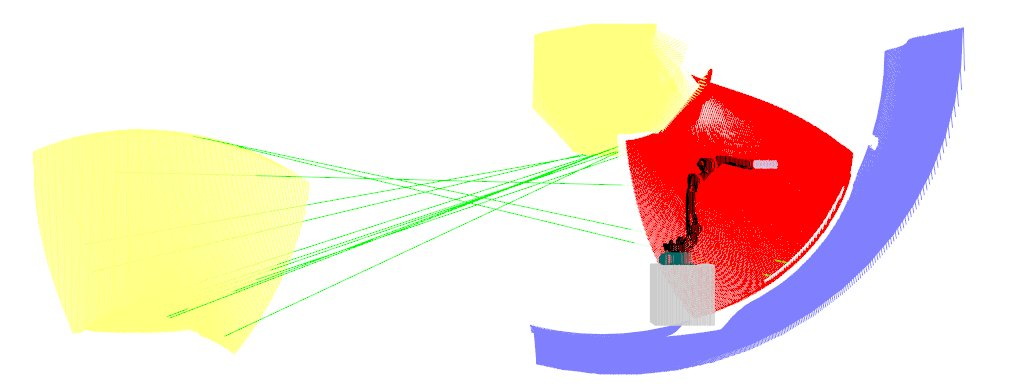
\includegraphics[width=.95\columnwidth]{figs/results/sim_mh12_sp}
    \caption{Robotic manipulator joints' torques in color gradient.}
    \label{fig:calibration}
\end{figure}